% !TeX spellcheck = cs_CZ
\wikitextrule
\begin{example}\label{fyz:fey_exam017}
  (Definiční obor a obor hodnot funkce): Určíme „co největší“ definiční obor funkce 
  \(y=\log_2{(\sqrt{1-x^2})}\) a zjistíme také její obor hodnot.
      
  {\centering
   \captionsetup{type=figure}
%   % !TeX spellcheck = cs_CZ
% exam017.tex
% K příkladu \ref{fyz:fey_exam017} \(y=\log_2{(\sqrt{1-x^2})}\) 

\documentclass[11pt]{standalone}
\usepackage{xltxtra}
\usepackage[usenames,x11names]{xcolor}
\usepackage{tikz}
\usepackage{pgfplots}
  \pgfplotsset{compat=newest}
\usepackage{amsmath}

\begin{document}
  \begin{tikzpicture}[thick,scale=0.7, every node/.style={transform shape}]
    \begin{axis}[
      xmin = -1, xmax = 1, ymin = -10, ymax = 0,
      domain = -0.999999:0.999999,
      restrict y to domain=-30:0,
      grid = major,   % both
      grid style={line width=.1pt, draw=gray!20},
      major grid style={dashed, line width=.2pt, draw=gray!40},
      minor tick num=5,
      clip = true,
      clip mode=individual,
      axis x line = middle,
      axis y line = middle,
      xlabel={\(x\)},
    %  xlabel style={at=(current axis.right of origin), anchor=west},
      ylabel={\(y\)},
    %  ylabel style={at=(current axis.above origin), anchor=south},
      enlarge y limits={rel=0.13},
      enlarge x limits={rel=0.07},
    ]
    
     \addplot[color=Gold3, samples=1000, smooth, ultra thick, unbounded coords=jump, no markers] 
        gnuplot{log10(sqrt(1-x^2))/log10(2)};  
    \end{axis}
  \end{tikzpicture}

\end{document}

% note: předchozí varianta MAI013
%\begin{tikzpicture}
%    \begin{axis}[
%        axis lines=middle,
%        width=10cm, height=10cm,     % size of the image
%        grid = both,
%        grid style={dashed, gray!30},
%        enlargelimits=true,
%        xmin=-1,      % start the diagram at this x-coordinate
%        xmax= 1,      % end   the diagram at this x-coordinate
%        ymin= -6,     % start the diagram at this y-coordinate
%        ymax= 0.5,     % end   the diagram at this y-coordinate
%        /pgfplots/xtick={-1,-0.5,...,1},   % make steps of length 0.2
%        /pgfplots/ytick={0,-0.5,...,-6},   % make steps of length 0.1
%        axis background/.style={fill=white},
%        axis line style={thick, shorten >=2pt, ->, > = {Latex[scale=1.3]}},
% %       every axis x label/.style={
% %        at={(ticklabel* cs:1.0)},
% %        anchor=west,
% %       },
% %       every axis y label/.style={
% %        at={(ticklabel* cs:1.0)},
% %        anchor=south,
% %       },
%        every axis x label/.style={at={(current axis.right of origin)},anchor=west},
%        every axis y label/.style={at={(current axis.north)},above=0mm},
%        ylabel=\(y\),
%        xlabel=\(x\),
% %       title={Dirichletova funkce}
%      ]
%      \addplot[domain=-0.9999:0.9999, line width=0.5pt,samples=1000,red]{log2(sqrt(1-x^2))};
%    \end{axis} 
%\end{tikzpicture}
   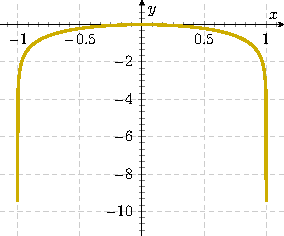
\includegraphics[width=0.4\linewidth]{mai_fig004.pdf}
   \captionof{figure}{K příkladu \ref{fyz:fey_exam017} \(y=\log_2{(\sqrt{1-x^2})}\) 
   \cite[s.~57]{Musilova2009MA1}
   \label{mai:fig004}}
  \par}
  
  Využijeme našich znalostí ze střední školy. Ve hře jsou tři funkce: logaritmus, odmocnina a 
  kvadratická funkce, postupně: 
  \begin{equation*}
    y = \log_2w, \qquad w = \sqrt{u}, \qquad u = 1 - x^2.
  \end{equation*}
  „Největším“ definičním oborem logaritmu je množina \(\mathcal{D}(log) = {w\realset \mid w > 0}\).
  Oborem hodnot logaritmu pro \(w \in \mathcal{D}(log)\) je celá reálná osa. Hodnoty \(w\) však 
  dostáváme vyčíslením odmocniny, která pro přípustné hodnoty \(u\), \(\mathcal{D}(\sqrt{ }) = 
  \lbrace u\in\realset | u\geq 0\rbrace\), může nabývat všech nezáporných hodnot, tj. kladných a 
  hodnoty nula (té nabývá pro \(u = 0\)). Hodnotu \(w = 0\) však nesmíme do logaritmu dosadit, 
  takže hodnotu \(u = 0\) musíme ihned vyloučit. Hodnoty proměnné \(x\) musíme omezit tak, aby 
  kvadratická funkce \(u = 1 — x^2\) nabývala pouze kladných hodnot. Dostáváme tak definiční obor 
  funkce \(y = f(x)\) \(\mathcal{D}=\lbrace x\in\realset | -1<x<1\rbrace\), neboli otevřený 
  interval \((—1, 1)\). Pro \(x \in \mathcal{D}\) pak funkce \(u(x)\) nabývá hodnot v          
  intervalu \(\mathcal{H}_u = \left( 0, 1\right]\) a funkce \(\log_2\sqrt{1-x^2}\) hodnot v 
  intervalu \(\mathcal{H}_u = \left( -\infty, 0\right]\), který je tedy jejím oborem hodnot. Graf 
  funkce vidíme na obr. \ref{mai:fig004}. 
\end{example}